\subsection*{Assignment 1 -- Data Understanding}
L'Assignment 1 richiedeva di esplorare il dataset originale,
soffermandosi su dati mancanti e possibili integrazioni con fonti
esterne di dati.\\

Il dataset originale era una aggregazione di dati ottenuti da diversi
servizi di streaming musicale; i dati erano inizialmente divisi in due
file distinti:
\begin{itemize}
    \item \texttt{tracks.json}, contenente informazioni relative alle
    canzoni,
    \item \texttt{artists.xml}, contenente informazioni relative agli
    artisti.
\end{itemize}

Per uniformare i formati e semplificare le operazioni di parsing e
integrazione, il file \texttt{artists.xml} è stato convertito in formato
JSON, ritenuto più adatto alla gestione programmatica rispetto a XML.
Fino alla successiva conversione in CSV, il dataset è stato quindi
manipolato utilizzando file JSON e dizionari Python.\\

\subsubsection*{Entità ed Attributi Principali}
Il dataset era costruito attorno ai suddetti artisti e canzoni.
La relazione tra queste due entità descriveva la partecipazione di
un artista alla produzione e pubblicazione di una canzone, e definiva
due modalità separate:
ogni canzone aveva un unico artista principale, e 0 o più artisti
featured.
Inoltre, vengono definite diversi ulteriori attributi ed entità,
ritenuti centrali nella descrizione del dominio.\\

Per quanto riguarda le canzoni, i principali sono stati considerati i
seguenti:
\begin{itemize}
    \item Alcune misure di popolarità, la più importante delle quali
    era \texttt{streams@1month}, che misurava il numero di stream ad un
    mese dalla pubblicazione;
    \item I \textbf{lyrics} delle canzoni, con vari ulteriori attributi
    descrittivi;
    \item Le date di uscita delle canzoni, salvate separatamente
    negli attributi \texttt{year}, \texttt{month} e \texttt{day};
    \item Gli \textbf{album} contenenti le canzoni, di diversi tipi
    (Singoli, Compilation ed Album). La loro descrizione era ulteriormente
    arricchita dalla presenza di vari attributi aggiuntivi.
    Seppure gli album non siano mai stati utilizzati nello studio,
    la loro rilevanza nella definizione e descrizione del dominio è
    stata ritenuta alta;
    \item Varie informazioni aggiuntive su aspetti più tecnici (dai BPM,
    Beats-Per-Minute, ad aspetti relativi ai file audio).
\end{itemize}

Il grafico sottostante mostra la distribuzione dell'attributo
\texttt{streams@1month}, che è stato il più rilevante durante tutto
il progetto.

\begin{figure}[h]
    \centering
    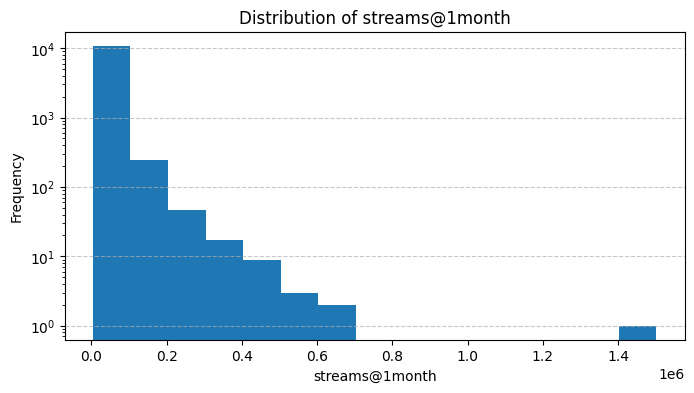
\includegraphics[width=0.7\textwidth]{Figures/streams_plot.png}
    \caption{Caption describing the figure}
    \label{fig:example}
\end{figure}


\subsubsection*{Dati Mancanti ed Errati}
Il dataset originale conteneva un alto numero di dati mancanti ed
incongruenze nella definizione degli attributi.

\subsubsection*{Dati Esterni}